\documentclass[notes,11pt, aspectratio=169]{beamer}

\usepackage{pgfpages}
% These slides also contain speaker notes. You can print just the slides,
% just the notes, or both, depending on the setting below. Comment out the want
% you want.
\setbeameroption{hide notes} % Only slide
%\setbeameroption{show only notes} % Only notes
%\setbeameroption{show notes on second screen=right} % Both

%\usepackage[scaled=1.0]{helvet}
\usepackage{array}


\usepackage{tikz}
\usepackage{verbatim}
\setbeamertemplate{note page}{\pagecolor{gray!5}\insertnote}
\usetikzlibrary{positioning}
\usetikzlibrary{snakes}
\usetikzlibrary{calc}
\usetikzlibrary{arrows}
\usetikzlibrary{decorations.markings}
\usetikzlibrary{shapes.misc}
\usetikzlibrary{matrix,shapes,arrows,fit,tikzmark}
\usepackage{amsmath}
\usepackage{mathpazo}
\usepackage{hyperref}
\usepackage{lipsum}
\usepackage{multimedia}
\usepackage{graphicx}
\usepackage{multirow}
\usepackage{graphicx}
\usepackage{dcolumn}
\usepackage{bbm}
\newcolumntype{d}[0]{D{.}{.}{5}}

\usepackage{changepage}
\usepackage{appendixnumberbeamer}
\newcommand{\beginbackup}{
   \newcounter{framenumbervorappendix}
   \setcounter{framenumbervorappendix}{\value{framenumber}}
   \setbeamertemplate{footline}
   {
     \leavevmode%
     \hline
     box{%
       \begin{beamercolorbox}[wd=\paperwidth,ht=2.25ex,dp=1ex,right]{footlinecolor}%
%         \insertframenumber  \hspace*{2ex} 
       \end{beamercolorbox}}%
     \vskip0pt%
   }
 }
\newcommand{\backupend}{
   \addtocounter{framenumbervorappendix}{-\value{framenumber}}
   \addtocounter{framenumber}{\value{framenumbervorappendix}} 
}


\usepackage{graphicx}
\usepackage[space]{grffile}
\usepackage{booktabs}

% These are my colors -- there are many like them, but these ones are mine.
\definecolor{blue}{RGB}{0,114,178}
\definecolor{red}{RGB}{213,94,0}
\definecolor{yellow}{RGB}{240,228,66}
\definecolor{green}{RGB}{0,158,115}

\hypersetup{
  colorlinks=false,
  linkbordercolor = {white},
  linkcolor = {blue}
}


%% I use a beige off white for my background
\definecolor{MyBackground}{RGB}{255,253,218}

%% Uncomment this if you want to change the background color to something else
%\setbeamercolor{background canvas}{bg=MyBackground}

%% Change the bg color to adjust your transition slide background color!
\newenvironment{transitionframe}{
  \setbeamercolor{background canvas}{bg=white}
  \begin{frame}}{
    \end{frame}
}

\setbeamercolor{frametitle}{fg=blue}
\setbeamercolor{title}{fg=black}
\setbeamertemplate{footline}[frame number]
\setbeamertemplate{navigation symbols}{} 
\setbeamertemplate{itemize items}{-}
\setbeamercolor{itemize item}{fg=blue}
\setbeamercolor{itemize subitem}{fg=blue}
\setbeamercolor{enumerate item}{fg=blue}
\setbeamercolor{enumerate subitem}{fg=blue}
\setbeamercolor{button}{bg=MyBackground,fg=blue,}

%%% TIKZ STUFF
\tikzset{   
	every picture/.style={remember picture,baseline},
	every node/.style={anchor=base,align=center,outer sep=1.5pt},
	every path/.style={thick},
}
\newcommand\marktopleft[1]{%
	\tikz[overlay,remember picture] 
	\node (marker-#1-a) at (-.3em,.3em) {};%
}
\newcommand\markbottomright[2]{%
	\tikz[overlay,remember picture] 
	\node (marker-#1-b) at (0em,0em) {};%
}
\tikzstyle{every picture}+=[remember picture] 
\tikzstyle{mybox} =[draw=black, very thick, rectangle, inner sep=10pt, inner ysep=20pt]
\tikzstyle{fancytitle} =[draw=black,fill=red, text=white]
%%%% END TIKZ STUFF


% If you like road maps, rather than having clutter at the top, have a roadmap show up at the end of each section 
% (and after your introduction)
% Uncomment this is if you want the roadmap!
% \AtBeginSection[]
% {
%    \begin{frame}
%        \frametitle{Roadmap of Talk}
%        \tableofcontents[currentsection]
%    \end{frame}
% }
\setbeamercolor{section in toc}{fg=blue}
\setbeamercolor{subsection in toc}{fg=red}
\setbeamersize{text margin left=1em,text margin right=1em} 

\newenvironment{wideitemize}{\itemize\addtolength{\itemsep}{10pt}}{\enditemize}
\newenvironment{wideenumerate}{\enumerate\addtolength{\itemsep}{10pt}}{\endenumerate}

\usepackage{environ}
\NewEnviron{videoframe}[1]{
  \begin{frame}
    \vspace{-8pt}
    \begin{columns}[onlytextwidth, T] % align columns
      \begin{column}{.58\textwidth}
        \begin{minipage}[t][\textheight][t]
          {\dimexpr\textwidth}
          \vspace{8pt}
          \hspace{4pt} {\Large \sc \textcolor{blue}{#1}}
          \vspace{8pt}
          
          \BODY
        \end{minipage}
      \end{column}%
      \hfill%
      \begin{column}{.42\textwidth}
        \colorbox{green!20}{\begin{minipage}[t][1.2\textheight][t]
            {\dimexpr\textwidth}
            Face goes here
          \end{minipage}}
      \end{column}%
    \end{columns}
  \end{frame}
}

\title[]{\textcolor{blue}{ECN 453: Pricing and Price Discrimination 1}}
\author[PGP]{}
\institute[FRBNY]{\small{\begin{tabular}{c c c}
Nicholas Vreugdenhil \\
\end{tabular}}}
\date{} 

\begin{document}

% Title Slide
\begin{frame}
\maketitle
  \centering
\end{frame}

% INTRO

\begin{frame}{Price Discrimination}
\begin{wideitemize}
	\item Price discrimination: \textbf{setting different prices for the same good}.
	\item Examples: airline tickets, software, pharmaceuticals
	\vspace{-10pt}
	\begin{figure}
	\item \includegraphics[scale=0.13]{airline.jpeg}
	\caption{Photo: Flickr/Victor}
	\end{figure}
	\item We will look at different ways that firms price discriminate and the implications for policy.
	%\item One surprising outcome we will discuss is that sometimes price discrimination can make consumers better off (!)
\end{wideitemize}
\end{frame}

\begin{frame}{Plan}
  \begin{wideenumerate}
  	\item Why price discriminate?
  	\item Price discrimination: selection by indicators
  	\item Price discrimination: self-selection
  	\item Non-linear pricing
  	\item Should price discrimination be legal?
  \end{wideenumerate}
\end{frame}

\begin{frame}{Plan}
	\begin{wideenumerate}
		\item \textbf{Why price discriminate?}
		\item Price discrimination: selection by indicators
		\item Price discrimination: self-selection
		\item Non-linear pricing
		\item Should price discrimination be legal?
	\end{wideenumerate}
\end{frame}

\begin{frame}{Why price discriminate?}
		\begin{wideitemize}
			\item Previously, we studied a monopolist who could only set \textbf{one price}.
			\item In the following diagram, I argue that a monopolist could increase profit if it could set \textbf{different prices for different consumers}.
		\end{wideitemize}
\end{frame}

\begin{frame}{Why price discriminate?: Monopoly diagram}
	\begin{figure}
		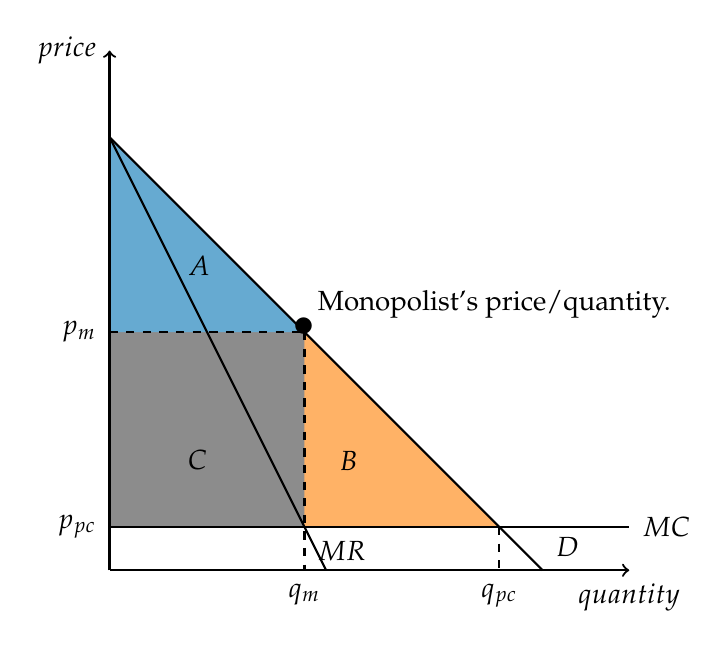
\begin{tikzpicture}[scale=0.55]
			\fill [darkgray!60] (0,1) -- (0,5.5) -- (4.5,5.5) -- (5.5,1) -- cycle;
			\fill [blue!60] (0,5.5) -- (4.5,5.5) -- (0,10) -- cycle;
			\fill [orange!60] (4.5,1) -- (4.5,5.5) -- (9,1) -- cycle;
			
			%y axis.....................
			\draw [->] (0,0) to (0,12) node [left] {$price$};
			
			%x axis......................
			\draw [->] (0,0) to (12,0) node [below] {$quantity$};
			
			% D curve...................
			\draw [thick] (0,10)  to  (10,0)  node [above right] {$D$};
			
			% MR curve....................
			\draw [thick] (0,10) to (5,0);
			\node [above right] at (4.5,-0.1) {$MR$};
			
			% MC=S curve...................
			\draw [thick] (0,1)  to  (12,1)  node [right] {$MC$};
			
			% dashed lines to equilibrium.............
			\draw [dashed] (0,5.5) node [left] {$p_m$} to (4.55,5.5); 
			\draw [dashed] (4.5,5.5) to (4.5,0) node [below] {$q_m$};
			
			% dashed lines to new equilibrium.........
			\draw [dashed] (0,1) node [left] {$p_{pc}$} to (9,1); 
			\draw [dashed] (9,1) to (9,0) node [below] {$q_{pc}$};
			
			% equilibrium points.......................
			\node [black] at (4.5,5.25) {\LARGE \textbullet};
			
			% labels..............................
			\node [black, above right] at (4.5,5.5) {Monopolist's price/quantity.};
			\node [above right] at (1.5,6.5) {$A$};
			\node [above right] at (5,2) {$B$};
			\node [above right] at (1.5,2) {$C$};
		\end{tikzpicture}
	\end{figure}
\end{frame}

\begin{frame}{Why price discriminate?: Monopoly diagram}
	\begin{wideitemize}
		\item On the previous slide there are three areas:
		\vspace{11pt}
	\end{wideitemize}
	\begin{wideenumerate}
		\item \textbf{Area A}: consumers who are willing to pay a price higher than $p_m$. 
			\begin{wideitemize}
				\item This was consumer surplus (when monopolist can only set one price)
				\item Monopolist could increase profits if it set \underline{higher prices} for these consumers.
			\end{wideitemize}
		\item \textbf{Area B}: consumers who are willing to pay a price lower than $p_m$, but higher than MC. 
			\begin{wideitemize}
				\item This was dead-weight-loss (when the monopolist can only set one price)
				\item The monopolist could increase profits if it set \underline{lower prices} for these consumers and sold to them.
			\end{wideitemize}
		\item \textbf{Area C}: this is the current profit of the monopolist.
	\end{wideenumerate}
\end{frame}

\begin{frame}{Why price discriminate?: Monopoly diagram}
		\begin{wideitemize}
			\item In order to fully extract all of area $A$ and $B$ in the previous diagram, the monopolist would have to know the \underline{exact willingness to pay} of each consumer in the market.
			\item This is called \textbf{perfect price discrimination}.
			\item Perfect price discrimination is a useful - but unrealistic - benchmark
			\item In practice, firms only have limited information about each consumer's willingness to pay. 
			\begin{wideitemize}
				\item We will now see some alternative forms of price discrimination when firms have more limited information about consumers.
			\end{wideitemize}
		\end{wideitemize}
\end{frame}

\begin{frame}{Plan}
	\begin{wideenumerate}
		\item Why price discriminate?
		\item \textbf{Price discrimination: selection by indicators}
		\item Price discrimination: self-selection
		\item Non-linear pricing
		\item Should price discrimination be legal?
	\end{wideenumerate}
\end{frame}

\begin{frame}{Price discrimination: selection by indicators}
	\begin{wideitemize}
		\item \textbf{Selection by indicators} is when the seller divides buyers into groups, setting a different price for each group.
		\item \textbf{Example:} Car sales
	\end{wideitemize}
	\begin{columns}[onlytextwidth, T] 
	\begin{column}{.5\textwidth}
		\begin{figure}
			\begin{tabular}{|c|c|c|}
				\hline
				Model & Italy & UK  \\
				\hline
				Fiat Uno& 21.7  & 8.7  \\
				Nissan Micra& 36.1  & 12.5  \\
				Mercedes 190 & 15.6  & 12.3  \\
				\hline
			\end{tabular}
			\caption{Car margins across countries}
		\end{figure}
	\end{column}
	\begin{column}{.5\textwidth}
				\begin{figure}
					\includegraphics[scale=0.12]{rav4.png}
				\end{figure}
			\end{column}
	\end{columns}
\end{frame}

\begin{frame}{Price discrimination: selection by indicators}
\begin{wideitemize}
	\item \textbf{Setup}:
	\item Two markets denoted 1 and 2.
	\item \underline{Demand}:
	\begin{wideitemize}
		\item market 1: $q_1=D_1(p_1)$ 
		\item market 2: $q_2=D_2(p_2)$
	\end{wideitemize}
	\item \underline{Total cost}: $C(Q)$ where the total quantity $Q$ is:
	 \begin{align*}
	 	Q=q_1 + q_2 =D_1(p_1) + D_2(p_2)
	\end{align*}
	%\item \underline{Total profit} $\Pi(p_1,p_2)$ is given by:
	%\begin{align*}
	%	\Pi(p_1,p_2) = p_1 D_1(p1) + p_2 D_2(p_2) - C(D_1(p1) + D_2(p_2))
	%\end{align*}
	\item \textbf{Question:} Find the optimal price (the profit maximizing price) in each market.
\end{wideitemize}
\end{frame}

\begin{frame}{Price discrimination: selection by indicators}
	\begin{wideitemize}
		\item \textbf{Solution}: Idea - \textbf{``two monopolists, one in each market''}
		\item \underline{Method 1:} The optimal price is where:
		\begin{align*}
			MR_1 = MC \text{ and } MR_2 = MC 
		\end{align*}
		\item In the above equation, $MR_1$ is marginal revenue in market 1, $MR_2$ is marginal revenue in market 2
		\item  \underline{Method 2:} Optimal prices must satisfy the elasticity rule:
		\begin{align*}
			p_1 (1+\frac{1}{\epsilon_1}) = MC \text{ and } 	p_2 (1+\frac{1}{\epsilon_2}) = MC
		\end{align*}
		\item In the above equation, $\epsilon_1$ and $\epsilon_2$ are the price elasticities of demand.
		%\item *(Optional math proving these results on the next slide, or you can just remember and apply the above results.)
	\end{wideitemize}
\end{frame}

\begin{frame}{Price discrimination: selection by indicators}
	\begin{wideitemize}
		\item Implication of optimal pricing under discrimination by market segmentation:
		\vspace{11pt}
		\begin{center}
			\textit{A seller should charge a lower price in those market segments with more elastic demand.}
		\end{center}
		\item Note: this statement can be a little confusing when you come to apply it because demand price elasticity is negative
		\begin{wideitemize}
			\item Just remember that `more elastic' means higher absolute values so that e.g. a market with $\epsilon=-4$ is more elastic than a market with $\epsilon=-2$
		\end{wideitemize}
		\item We will now see particular example of the above statement.
	\end{wideitemize}	
\end{frame}

\begin{frame}{Price discrimination: selection by indicators - example 1, p126}
\begin{wideitemize}
	\item \textbf{Setup:}
	\item Demand elasticities for market 1 and market 2: $\epsilon_1=-4, \epsilon_2=-2$.
	\item Marginal cost = 6
	\item \textbf{Question:} What are the optimal prices in market 1 and market 2?
	\item \textbf{Solution:} 
	\begin{wideitemize}
		\item Apply elasticity rule ($p_1 (1+\frac{1}{\epsilon_1}) = MC \text{ and } 	p_2 (1+\frac{1}{\epsilon_2}) = MC$):
		\begin{align*}
			p_1 ( 1 - 1/4) &= 6 \\
			p_2 (1- 1/2) &= 6
		\end{align*}
		\item Solving for $p_1$ and $p_2$ implies: $p_1=\$8, p_2=\$12$.
		\item Note that $p_1 < p_2$ since market 1 is more elastic than market 2.
	\end{wideitemize}
\end{wideitemize}
\end{frame}

\begin{frame}{Price discrimination: selection by indicators - example 2, p127}
	\begin{wideitemize}
		\item \textbf{Setup:}
		\item Market 1 demand: $q_1 = 12 - 2p_1$
		\item Market 2 demand: $q_2 = 4 -p_2$
		\item Marginal cost = 1
		\item \textbf{Questions:} 
		\item 1. What is the optimal uniform price? 
		\item 2. What are the optimal prices in each market when the monopolist can charge different prices in each market? 
		\item 3. How much does profit increase between 1. a uniform price vs 2. different prices?
	\end{wideitemize}
\end{frame}
\begin{frame}{Price discrimination: selection by indicators - example 2}
	\begin{wideitemize}
		\item \textbf{Solution:}
		\item 1. What is the optimal uniform price? 
		\begin{wideitemize}
			\vspace{11pt}
			\item Idea: combine the two markets to a single market with the same price $p=p_1=p_2$, and apply the usual monopoly solution.
			\item Total demand: $Q = q_1+q_2 = 12- 2 p_1 + 4 - p_2 = 16 -3p$
			\begin{wideitemize}
				\item Note: The above is true so long as demand in positive in both markets (i.e. here $p \leq 4$). If price is $> 4$ then the demand in market 2 will be 0 and total demand $Q=12-2p_1$. We will assume for now that demand is positive in both markets, and check that the final price $p \leq 4$.
			\end{wideitemize}
			\item Rearrange for price: $p = \frac{16}{3} - \frac{1}{3}Q$
			\item Get MR using `twice the slope trick': $MR = p = \frac{16}{3} - \frac{2}{3}Q$
			\item Use MR=MC and solve for optimal $Q$: $\frac{16}{3} - \frac{2}{3}Q = 1$. So, $Q=6.5$
			\item Solve for optimal price using $Q$: $p =  \frac{16}{3} - \frac{1}{3} \frac{13}{2} = 3.1667$
		\end{wideitemize}
	\end{wideitemize}
\end{frame}

\begin{frame}{Price discrimination: selection by indicators - example 2}
	\begin{wideitemize}
		\item \textbf{Solution:}
		\item 2. What are the optimal prices in each market when the monopolist can charge different prices in each market? 
		\begin{wideitemize}
			\vspace{11pt}
			\item \underline{Market 1}:
				\item  Demand: $q_1 = 12 - 2p_1$
				\item Rearrange for price: $p_1 = 6 - \frac{1}{2} q_1$
				\item Get $MR_1$ using `twice the slope trick': $MR_1 = 6 - q_1$
				\item Use $MR_1=MC$ and solve for optimal $q_1$: $6-q_1=1$, so $q_1=5$
				\item Plug in $q_1=5$ into demand to get price: $p_1 = 6 - \frac{1}{2} \times 5=3.5$
		\end{wideitemize}
	\end{wideitemize}
\end{frame}

\begin{frame}{Price discrimination: selection by indicators - example 2}
	\begin{wideitemize}
		\item \textbf{Solution:}
		\item 2. What are the optimal prices in each market when the monopolist can charge different prices in each market? 
		\begin{wideitemize}
			\vspace{11pt}
			\item \underline{Market 2}:
			\item  Demand: $q_2 = 4 - p_2$
			\item Rearrange for price: $p_2 = 4 - q_2$
			\item Get $MR_2$ using `twice the slope trick': $MR_2 = 4 - 2q_2$
			\item Use $MR_2=MC$ and solve for optimal $q_2$: $4-2q_2=1$, so $q_2=1.5$
			\item Plug in $q_2=1.5$ into demand to get price: $p_2=4 - 1.5=2.5$
		\end{wideitemize}
	\end{wideitemize}
\end{frame}

\begin{frame}{Price discrimination: selection by indicators - example 2}
	\begin{wideitemize}
		\item \textbf{Solution:}
		\item 3. How much does profit increase between 1. a uniform price vs 2. different prices?
		\begin{wideitemize}
			\vspace{11pt}
			\item Profit with uniform prices ($Q=6.5,p=3.1667$):
			\begin{align*}
				TR-TC = 6.5 \times 3.1667 - 6.5 \times 1 = 14.08 
			\end{align*}
			\item Profit with different prices ($q_1=5,p_1=3.5,q_2=1.5,p_2=2.5$)
			\begin{align*}
				\text{Market 1:}& \hspace{11pt} TR-TC = 5 \times 3.5 - 5 \times 1 = 12.5 \\
				\text{Market 2:}& \hspace{11pt} TR-TC = 1.5 \times 2.5 - 1.5 \times 1 = 2.25
			\end{align*}
			\item So, total profit with different prices $= 12.5+2.25 = 14.75$.
			\item Profit increases from $14.08$ to $14.75$ (i.e. by $0.67$) moving from uniform to different prices.
		\end{wideitemize}
	\end{wideitemize}
\end{frame}

\begin{frame}{Plan}
	\begin{wideenumerate}
		\item Why price discriminate?
		\item Price discrimination: selection by indicators
		\item \textbf{Price discrimination: self-selection}
		\item Non-linear pricing
		\item Should price discrimination be legal?
	\end{wideenumerate}
\end{frame}


\begin{frame}{Price discrimination: self-selection}
	\begin{wideitemize}
		\item In the previous section we studied `selection by indicators'.
		\begin{wideitemize}
			\vspace{11pt}
			\item To use selection by indicators, the seller needed information about the characteristics of consumers so they could offer different buyers different prices.
			\item Often, sellers do not have much information about consumers. 
			\item e.g. if you're selling airline tickets online, not much information about who the high-value business travellers are.
		\end{wideitemize}
		\item We will now discuss three types of \textbf{price discrimination by self-selection}.
		\begin{wideitemize}
			\vspace{11pt}
			\item These are used when the seller does not have much information about the characteristics of consumers.
			\item Instead, the seller offers different `deals' which cause buyers to self-select into which group they belong to.
		\end{wideitemize}
	\end{wideitemize}
\end{frame}

\begin{frame}{Self-selection: versioning}
	\begin{wideitemize}
		\item \textbf{Self-selection by versioning}: offering different `versions' of a product, each version targeted at a different group of consumers.
		\item Typical: a `high-quality' version targeted at high-value consumers, and a `lower-quality' version targeted at low-value consumers.
	\end{wideitemize}
    \begin{columns}[onlytextwidth, T] % align columns
		\begin{column}{.58\textwidth}
			\begin{wideitemize}
				\item \textbf{Examples:}
				\item Discount airfares with date/destination restrictions
				\item Iphone pro vs Iphone pro max
				\item Different models of Amazon Kindle
			\end{wideitemize}
		\end{column}
		\begin{column}{0.5\textwidth}
			\begin{centering}
				\includegraphics[scale=0.12]{iphone.png}
			\end{centering}	
		\end{column}
	\end{columns}
\end{frame}

\begin{frame}{Self-selection: versioning}
	\begin{wideitemize}
		\item An extreme form of versioning: \textbf{damaged goods} - reduce the quality of existing products
		\item \textbf{Example:}
	\end{wideitemize}
	\begin{columns}
		\begin{column}{0.4\textwidth}
			\begin{figure}
				\includegraphics[scale=0.2]{tesla.jpeg}
				\caption{2017 Tesla Model S full range: \$76 thousand}
			\end{figure}
		\end{column}
		\begin{column}{0.4\textwidth}
			\begin{figure}
				\includegraphics[scale=0.2]{tesla.jpeg}
				\caption{Exactly the same car with a few extra lines of code to restrict battery: \$70 thousand}
			\end{figure}
		\end{column}
	\end{columns}
		\begin{wideitemize}
			\item Why would it be profitable for a seller to intentionally make some of its products worse? Price discrimination.
		\end{wideitemize}
\end{frame}

\begin{frame}{Self-selection: versioning, example (p131)}
\begin{wideitemize}
	\item \textbf{Example:}
	\item Two versions of product: full and stripped-down. MC = 300 for both versions.
	\item Two types of consumers: 1 million people of type 1; 0.2 million people of type 2
	\item Willingness-to-pay of consumers:
	\begin{figure}
		\centering
	\begin{tabular}{|c|c|c|}
		\hline
		& full &stripped-down\\
		\hline
		type 1 (high-end)& 1500  & 800  \\
		type 2 (low-end)&600  & 500  \\
		\hline
	\end{tabular}
	\end{figure}
	\item \textbf{Questions:} 
	\item 1. Find the profit from selling only the full version for 1500.
	\item 2. Find the profit from charging 1500 for full version; 500 for the stripped-down version.
	\item 3. Find the profit from charging 1199 for full version; 500 for the stripped-down version.
\end{wideitemize}
\end{frame}

\begin{frame}{Self-selection: versioning, example}
	\begin{wideitemize}
		\item \textbf{Solution:}
		\item Idea: each type of consumer will \underline{self-select} into the version with the \underline{highest consumer surplus} (consumer surplus=willingness-to-pay - price). E.g. the consumers buy the full version if:
		\begin{align*}
			\text{consumer 1: } &1500-p_{full} > 800 - p_{stripped-down} \\
			\text{consumer 2: } &600-p_{full} > 500 - p_{stripped-down}
		\end{align*}
		\item 1. Find the profit from selling only the full version for 1500.
		\vspace{11pt}
		\begin{wideitemize}
			\item Consumer type 1 buys the full version (receiving CS=0)
			\item Consumer type 2 does not buy anything (since their CS would be 800-1500=-700 from buying the full version).
			\item Then, $Profit = (1500-300) \times 1 \text{ million} = \$1.2 \text{ billion}$
		\end{wideitemize}
	\end{wideitemize}
\end{frame}

\begin{frame}{Self-selection: versioning, example}
	\begin{wideitemize}
		\item \textbf{Solution:}
		\item 2. Find the profit from charging 1500 for full version; 500 for the stripped-down version.
		\vspace{11pt}
		\begin{wideitemize}
			\item (Why are we considering this pricing? This is the pricing the seller would choose if it could practice perfect price discrimination. That is, pricing the full version at the type-1 willingness-to-pay and the stripped-down version at the type-2 willingness-to-pay.)
			\item \underline{Consumer type 1:} buys stripped down version (CS=0 from full version but CS=800-500=300 from the stripped-down version).
			\item \underline{Consumer type 2:} buys stripped down version (CS=600-1500=-900 from full version but CS=500-500=0 from the stripped-down version).
			\item Then, $Profit = (500-300) \times 1 \text{ million} + (500-300) \times 0.2 \text{ million} = \$240 \text{ million}$
			\item Profit is actually less than in part 1 when we only offered the full version. Why? Consumer type 1 now chooses the stripped-down version.
		\end{wideitemize}
	\end{wideitemize}
\end{frame}

\begin{frame}{Self-selection: versioning, example}
	\begin{wideitemize}
		\item \textbf{Solution:}
		\item 3. Find the profit from charging 1199 for full version; 500 for the stripped-down version.
		\vspace{11pt}
		\begin{wideitemize}
			\item \underline{Consumer type 1:} buys full version (CS=1500-1199=301 from full version but CS=800-500=300 from the stripped-down version).
			\item \underline{Consumer type 2:} buys stripped down version (CS=600-1199=-599 from full version but CS=500-500=0 from the stripped-down version).
			\item Then, $Profit = (1200-300) \times 1 \text{ million} + (500-300) \times 0.2 \text{ million} = \$1.3 \text{ billion}$
			\item So, compared to Part 1, the seller is better off by \$100 million.
		\end{wideitemize}
	\end{wideitemize}
\end{frame}

\begin{frame}{Self-selection: versioning}
	\begin{wideitemize}
		\item Why are profits in Part 3 of the previous example higher than in Part 2?
		\item The reason is that the prices in Part 3 ensured that the \textbf{high-end consumer had no incentive to go for the deal that was intended for the low-end consumer.} 
		\begin{wideitemize}
			\vspace{11pt}
			\item Put another way, the prices in Part 3 of the example ensured that high-end consumers self-selected into buying the high-quality version, and low-end consumers self-selected into buying the low-quality version. 
		\end{wideitemize}
		\item We will now study another form of price discrimination by self-selection: bundling.
	\end{wideitemize}
\end{frame}

\begin{frame}{Self-selection: bundling}
	\begin{wideitemize}
		\item \textbf{Bundling}: combining products and selling them together.
	\end{wideitemize}
	\begin{columns}
		\begin{column}{0.4\textwidth}
		\begin{wideitemize}
		\item \textbf{Examples}: 
		\item Software is bundled as a `suite' e.g. microsoft office
		\item Cable tv channels
		\item Phone and internet plans
		\item Movie distribution
		\end{wideitemize}
		\end{column}
		\begin{column}{0.6\textwidth}
			\begin{figure}
			\vspace{11pt}
			\includegraphics[scale=0.12]{bundles.jpeg}
			\caption{Centurylink internet bundles}
			\end{figure}
		\end{column}
	\end{columns}
\end{frame}

\begin{frame}{Self-selection: bundling, example p133}
	\begin{wideitemize}
		\item \textbf{Example}: Three user types: writer, number cruncher, generalist. Two products: word processor, spreadsheet. Assume $TC =0$.
		\begin{table}
			\begin{tabular}{|l|c|c|c|}
				\hline
				\textbf{User type}&  \textbf{Number of users} & \multicolumn{2}{c}{\textbf{Willingness to pay}} \\
				\hline
				& & Word processor & Spreadsheet  \\
				\hline
				Writer& 40 & 50 & 0  \\
				\hline
				Number cruncher& 40  & 0 & 50  \\
				\hline
				Generalist& 20  & 30 & 30  \\
				\hline
			\end{tabular}
		\end{table}
		\item \textbf{Questions}:
		\item 1. What is the profit if each product is sold separately?
		\item 2. What is the profit if each product is sold separately for \$50 \underline{and} a bundle of the two products is offered for \$60?
	\end{wideitemize}
\end{frame}

\begin{frame}{Self-selection: bundling, example p133}
\begin{wideitemize}
	\item Main idea: each consumer will choose (i.e. self-select into) the product/bundle with the highest consumer surplus (= willingness-to-pay - price). We need to first find the optimal price and then find the profit.
	\item 1. What is the profit if each product is sold separately?
	\item \textbf{Solution:}
	\item The optimal price is to charge \$50 for the word processor and \$50 for the spreadsheet.
	\begin{wideitemize}
			\item Here, writers choose the word processor (and generate profit $= 50 \times 40 = \$2000$), and number crunchers choose the spreadsheet (generating \$2000), for \underline{total profit of \$4000}.
	\end{wideitemize}
	\item An alternative price is to charge \$30 for both products. But, this is not optimal.
	\begin{wideitemize}
		\item Both writers and generalists will choose the word processor (generating $40 \times 30 + 20 \times 30 = \$1800$ from word processors). Similarly, \$1800 profit is made from selling the spreadsheet for a total profit of \$3600.
	\end{wideitemize}
	\item (If it's not obvious, convince yourself that intermediate prices e.g. \$40 for both products, are not optimal.)
\end{wideitemize}
\end{frame}

\begin{frame}{Self-selection: bundling, example p133}
	\begin{wideitemize}
		\item 2. What is the profit if each product is sold separately for $\$50$ \underline{and} a bundle of the two products is offered for \$60?
		\item \textbf{Solution:}
		\item \underline{Writers:} choose the word processor (they could choose the bundle but they would be paying \$10 more for something they do not value). Profit from writers = $40 \times 50 = 2000$.
		\item \underline{Number cruncher:} choose the spreadsheet (they could choose the bundle but they would be paying \$10 more for something they do not value). Profit from number crunchers = $40 \times 50 = 2000$.
		\item \underline{Generalists:} choose the bundle (value the bundle at \$60, but would not want to buy a word processor or spreadsheet individually for \$50 since they only value each of these at \$30). Profit from generalists = \$1800.
		\item So, make \$5800 profit in total, and \$1800 more profit, from selling the bundle.
	\end{wideitemize}
\end{frame}

\begin{frame}{Self-selection: bundling, example p133}
		\begin{wideitemize}
			\item Why did bundling increase profits in the previous example?
			\item By offering a bundle of the two products, the seller was able to:
			\begin{wideitemize}
				\item get the generalist group to self-select into buying the bundle...
				\item ...while still getting the writers and number crunchers to purchase products separately.
			\end{wideitemize}
			\item This self-selection revealed to the seller the type of user. 
			\begin{wideitemize}
				\item The seller could then price-discriminate and charge a price equal to the willingness-to-pay in each group.
			\end{wideitemize}
\end{wideitemize}
\end{frame}

\begin{frame}{Plan}
	\begin{wideenumerate}
		\item Why price discriminate?
		\item Price discrimination: selection by indicators
		\item Price discrimination: self-selection
		\item \textbf{Non-linear pricing}
		\item Should price discrimination be legal?
	\end{wideenumerate}
\end{frame}

\begin{frame}{Non-linear pricing}
\begin{columns}
	\begin{column}{0.6\textwidth}
		\begin{wideitemize}
			\item Consumers often decide not just \textit{whether} to buy a produce but also \textit{how much}.
			\item \textbf{Examples}
			\begin{wideitemize}
				\item How many scoops of ice-cream?
				\item How much electricity/water/gas to use?
			\end{wideitemize}
			\item \textbf{Non-linear pricing}: when the price changes with the total quantity purchased.
			\begin{wideitemize}
				%\item As we will see, this is another example of `price discrimination by self-selection', but following the book I present it in its own section.
				\item e.g. first ice-cream scoop costs \$5, second costs \$2, third \$1,...
			\end{wideitemize}
		\end{wideitemize}
	\end{column}
	\begin{column}{0.4\textwidth}
	\begin{figure}
		\includegraphics[scale=0.15]{icecream.jpeg}
		\caption{Getty Images}
	\end{figure}
	\end{column}
\end{columns}
\end{frame}

\begin{frame}{Non-linear pricing}
	\begin{wideitemize}
		\item We will look at a particular form of non-linear pricing: \textbf{two-part tariffs} 
		\begin{wideitemize}
			\item We will study the case with homogeneous consumers (i.e. identical consumers who all have the same demand curve). Technically, this is not an example of price discrimination but rather more general pricing strategies - it is in this section to be consistent with the textbook.
		\end{wideitemize}
		\item A two-part tariff is in the form: 
		\begin{align*}
			\text{two-part tariff = }f + pq
		\end{align*}
		%\item Where:
		\begin{wideitemize}
			\item $f$: fixed part (e.g. golf club membership)
			\item $p$: variable part (e.g. greens fee you pay every time you play golf)
			\item $q$: quantity
		\end{wideitemize}
		\item The \textbf{price per unit} (i.e. average price) is $p+f/q$ and decreases as quantity $q$ increases.
		\item We will see how a two-part tariff can be more profitable for a seller than a single price.
	\end{wideitemize}
\end{frame}

\begin{frame}{Non-linear pricing: how should the seller choose $f$ and $p$?}
	\begin{columns}
		\begin{column}{0.5\textwidth}
			\begin{figure}
			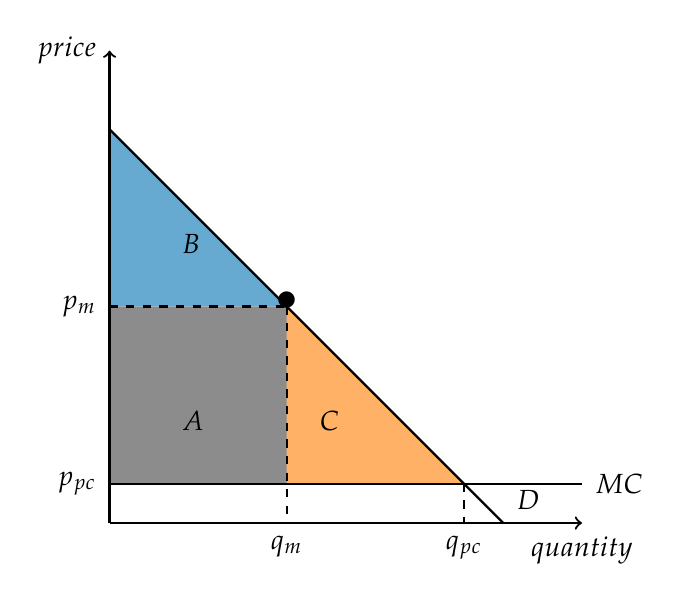
\begin{tikzpicture}[scale=0.5]
				\fill [darkgray!60] (0,1) -- (0,5.5) -- (4.5,5.5) -- (5.5,1) -- cycle;
				\fill [blue!60] (0,5.5) -- (4.5,5.5) -- (0,10) -- cycle;
				\fill [orange!60] (4.5,1) -- (4.5,5.5) -- (9,1) -- cycle;
				
				%y axis.....................
				\draw [->] (0,0) to (0,12) node [left] {$price$};
				
				%x axis......................
				\draw [->] (0,0) to (12,0) node [below] {$quantity$};
				
				% D curve...................
				\draw [thick] (0,10)  to  (10,0)  node [above right] {$D$};
				
				% MR curve....................
				%\draw [thick] (0,10) to (5,0);
				%\node [above right] at (4.5,-0.1) {$MR$};
				
				% MC=S curve...................
				\draw [thick] (0,1)  to  (12,1)  node [right] {$MC$};
				
				% dashed lines to equilibrium.............
				\draw [dashed] (0,5.5) node [left] {$p_m$} to (4.55,5.5); 
				\draw [dashed] (4.5,5.5) to (4.5,0) node [below] {$q_m$};
				
				% dashed lines to new equilibrium.........
				\draw [dashed] (0,1) node [left] {$p_{pc}$} to (9,1); 
				\draw [dashed] (9,1) to (9,0) node [below] {$q_{pc}$};
				
				% equilibrium points.......................
				\node [black] at (4.5,5.25) {\LARGE \textbullet};
				
				% labels..............................
				%\node [black, above right] at (4.5,5.5) {Monopolist's price/quantity.};
				\node [above right] at (1.5,6.5) {$B$};
				\node [above right] at (5,2) {$C$};
				\node [above right] at (1.5,2) {$A$};
			\end{tikzpicture}
			\end{figure}
		\end{column}
		\begin{column}{0.5\textwidth}
			\begin{wideitemize}
				\item First, find optimal $f$ \underline{given a particular} price $p$ (e.g. $p=p_m$, the monopoly price)
				\begin{wideitemize}
					\item Recall that area B is the consumer surplus for a particular price p (denote this $CS(p)$). 
					\item It is optimal to set $f=CS(p)$.
					\item Why? If $f > CS(p)$ then noone will buy.
					\item If $f < CS(p)$ then the seller is leaving money on the table.
				\end{wideitemize}
				\item Recall that area A is the seller's (variable) profit.
				\item So, the seller's total profits = A + B.
			\end{wideitemize}
		\end{column}
	\end{columns}
\end{frame}

\begin{frame}{Non-linear pricing: how should the seller choose $f$ and $p$?}
		\begin{columns}
		\begin{column}{0.5\textwidth}
			\begin{figure}
				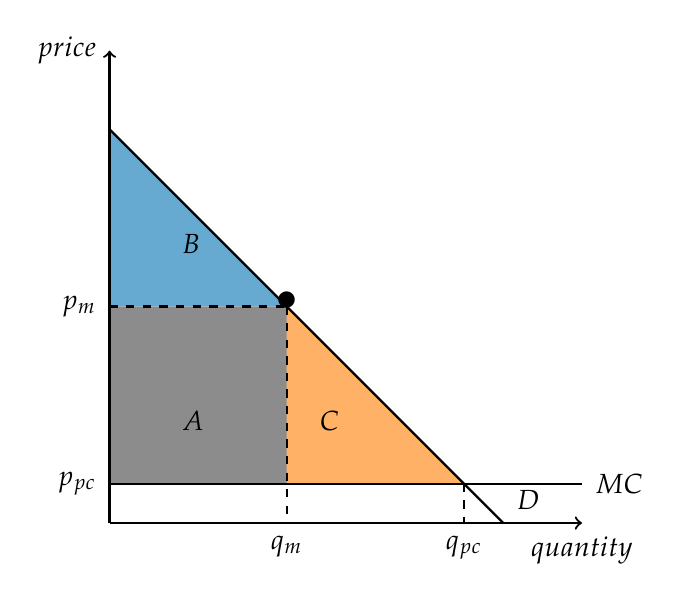
\begin{tikzpicture}[scale=0.5]
					\fill [darkgray!60] (0,1) -- (0,5.5) -- (4.5,5.5) -- (5.5,1) -- cycle;
					\fill [blue!60] (0,5.5) -- (4.5,5.5) -- (0,10) -- cycle;
					\fill [orange!60] (4.5,1) -- (4.5,5.5) -- (9,1) -- cycle;
					
					%y axis.....................
					\draw [->] (0,0) to (0,12) node [left] {$price$};
					
					%x axis......................
					\draw [->] (0,0) to (12,0) node [below] {$quantity$};
					
					% D curve...................
					\draw [thick] (0,10)  to  (10,0)  node [above right] {$D$};
					
					% MR curve....................
					%\draw [thick] (0,10) to (5,0);
					%\node [above right] at (4.5,-0.1) {$MR$};
					
					% MC=S curve...................
					\draw [thick] (0,1)  to  (12,1)  node [right] {$MC$};
					
					% dashed lines to equilibrium.............
					\draw [dashed] (0,5.5) node [left] {$p_m$} to (4.55,5.5); 
					\draw [dashed] (4.5,5.5) to (4.5,0) node [below] {$q_m$};
					
					% dashed lines to new equilibrium.........
					\draw [dashed] (0,1) node [left] {$p_{pc}$} to (9,1); 
					\draw [dashed] (9,1) to (9,0) node [below] {$q_{pc}$};
					
					% equilibrium points.......................
					\node [black] at (4.5,5.25) {\LARGE \textbullet};
					
					% labels..............................
					%\node [black, above right] at (4.5,5.5) {Monopolist's price/quantity.};
					\node [above right] at (1.5,6.5) {$B$};
					\node [above right] at (5,2) {$C$};
					\node [above right] at (1.5,2) {$A$};
				\end{tikzpicture}
			\end{figure}
		\end{column}
		\begin{column}{0.5\textwidth}
			\begin{wideitemize}
				\item We still need to optimally choose the variable part $p$.
				\item In the previous slide we saw that optimally choosing the fixed part $f$ results in the total profit = A + B.
				\item So, let's choose $p$ to make the area A + B as big as possible.
				\item This happens at $p=p_{pc}$ i.e. the perfect competition price.
			\end{wideitemize}
		\end{column}
	\end{columns}
\end{frame}

\begin{frame}{Non-linear pricing: how should the seller choose $f$ and $p$?}
	\begin{wideitemize}
	\item The \textbf{optimal two-part tariff} (with identical consumers) is:
			\item Set $p=p_{pc}$ (the perfect competition price)
			\item Set $f=CS(p_{pc})= \text{A + B + C}$ (i.e. total surplus under perfect competition)
			\item Note: areas A, B, C displayed on the previous slide
	\end{wideitemize}
\end{frame}

\begin{frame}{Non-linear pricing: efficiency and equity}
		\begin{wideitemize}
			\item Who were the winners and losers from moving from uniform pricing (i.e. the monopoly price) to a two-part tariff?
			\begin{wideitemize}
				\item \textbf{Winner:} the sellers; profits increased from $A$ to $A+B+C$.
				\item \textbf{Loser:} consumers; consumer surplus decreased from $B$ to $0$.
			\end{wideitemize}
			\item Overall, the two-part tariff is more \textbf{efficient}. 
			\begin{wideitemize}
				\item Total surplus increases from $A+B$ to $A+B+C$. In fact, it completely eliminated all of the (inefficient) dead-weight-loss of the monopolist (area B).
			\end{wideitemize}
			\item However, this came at the cost of \textbf{equity}: consumer surplus was reduced to 0.
		\end{wideitemize}
\end{frame}

\begin{frame}{Plan}
	\begin{wideenumerate}
		\item Why price discriminate?
		\item Price discrimination: selection by indicators
		\item Price discrimination: self-selection
		\item Non-linear pricing
		\item \textbf{Should price discrimination be legal?}
	\end{wideenumerate}
\end{frame}

\begin{frame}{Should price discrimination be legal?}
	\begin{columns}
		\begin{column}{0.4\textwidth}
			\begin{figure}
				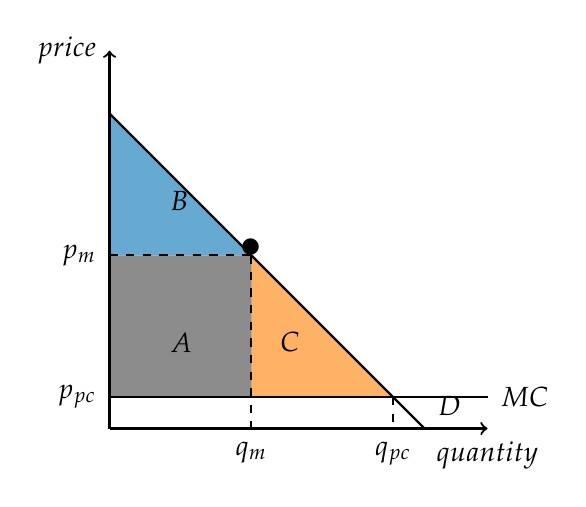
\begin{tikzpicture}[scale=0.4]
					\fill [darkgray!60] (0,1) -- (0,5.5) -- (4.5,5.5) -- (5.5,1) -- cycle;
					\fill [blue!60] (0,5.5) -- (4.5,5.5) -- (0,10) -- cycle;
					\fill [orange!60] (4.5,1) -- (4.5,5.5) -- (9,1) -- cycle;
					
					%y axis.....................
					\draw [->] (0,0) to (0,12) node [left] {$price$};
					
					%x axis......................
					\draw [->] (0,0) to (12,0) node [below] {$quantity$};
					
					% D curve...................
					\draw [thick] (0,10)  to  (10,0)  node [above right] {$D$};
					
					% MR curve....................
					%\draw [thick] (0,10) to (5,0);
					%\node [above right] at (4.5,-0.1) {$MR$};
					
					% MC=S curve...................
					\draw [thick] (0,1)  to  (12,1)  node [right] {$MC$};
					
					% dashed lines to equilibrium.............
					\draw [dashed] (0,5.5) node [left] {$p_m$} to (4.55,5.5); 
					\draw [dashed] (4.5,5.5) to (4.5,0) node [below] {$q_m$};
					
					% dashed lines to new equilibrium.........
					\draw [dashed] (0,1) node [left] {$p_{pc}$} to (9,1); 
					\draw [dashed] (9,1) to (9,0) node [below] {$q_{pc}$};
					
					% equilibrium points.......................
					\node [black] at (4.5,5.25) {\LARGE \textbullet};
					
					% labels..............................
					%\node [black, above right] at (4.5,5.5) {Monopolist's price/quantity.};
					\node [above right] at (1.5,6.5) {$B$};
					\node [above right] at (5,2) {$C$};
					\node [above right] at (1.5,2) {$A$};
				\end{tikzpicture}
			\end{figure}
		\end{column}
		\begin{column}{0.6\textwidth}
\begin{wideitemize}
	\item The non-linear pricing figure from the previous section also depicts the welfare effects of moving from uniform pricing to perfect price discrimination.
	\item Allowing price discrimination typically:
	\begin{wideitemize}
		\item Increases total surplus ($A+B \rightarrow A+B+C$)
		\item Reduces consumer surplus ($B \rightarrow 0$)
		\begin{wideitemize}
			\item Note: it is possible to construct examples where consumers to be better off under price discrimination, but in most of the cases we will see they are worse off.
		\end{wideitemize}
		\item Results in more consumers being served ($q_m \rightarrow q_{pc}$)
	\end{wideitemize}
\end{wideitemize}
		\end{column}
	\end{columns}
\end{frame}

\begin{frame}{Should price discrimination be legal?}
	\begin{wideitemize}
		\item Whether to allow price discrimination often comes down to an \textbf{equity-efficiency tradeoff}.
		\begin{wideitemize}
			\vspace{11pt}
			\item Policymakers may still want to prevent pricing strategies that are efficient for equity reasons. 
		\end{wideitemize}
	\end{wideitemize}
		\begin{wideitemize}
						\vspace{11pt}
			\item While economics makes precise predictions about overall efficiency and the winners/losers from a policy, it usually has less to say about how society should best trade-off these competing objectives.
		\end{wideitemize}
\end{frame}



\end{document}